\documentclass[a4paper, 12pt]{article}
\usepackage{listings} 
\usepackage{xcolor}
\usepackage{mdframed}
\usepackage{graphicx}
\definecolor{code-gray}{gray}{0.93}
\begin{document}
\title{ECE 341 - Lab \#6}
\author{Collin Heist}
\date{\today}
\maketitle
\pagenumbering{roman}
\tableofcontents
\lstlistoflistings
\newpage
\pagenumbering{arabic}

\section{Introduction}
The purpose of this lab is to become familiar with using the LCD, as well as the basics of interfacing with a peripheral operating at a different clock speed than the Micro-controller. We'll be using the PmodCLP (LCD), and communicating with it through our board's \textbf{PMP} peripheral. Our goal is to write a general-purpose LCD interface library, with 6 primary functions, and then test the functionality of that library with a basic string of text we'll alternate every 5 seconds.

The \textbf{PMP} is the only new peripheral for this week's lab, and it's a configurable peripheral with a variable amount of parallel data lines, a multiplexed address bus, and some control lines (enable, read, write). The \textbf{PMP} is meant for use with a wide variety of devices, not just the LCD that we'll be using it for here. Examples of other uses for this peripheral are external memory devices (given the limited memory of the PIC32), other peripherals, and even slave micro-controllers. 

We'll be using the \textbf{PMP} on our PIC32 to communicate not \textit{directly} with the LCD, but with the LCD's controller. This is functionall equivalent, except the LCD controller handles all the 'nitty-gritty' display of the LCD itself. This is because the LCD is broken up into many pixels, and each ASCII character corresponds to some visual combination of those characters. Rather than addressing the LCD with the very tedious pixel-by-pixel communications, the LCD controller takes the ASCII character, or instruction if we're configuring the LCD, and handles the tedious control of the individual pixels for us. This reduces the development time necessary for writing to an LCD, and only requires that the LCD controller and LCD screen be configured together.

\section{Implementation}
To begin the lab, I created the header file for interfacing with the LCD. Because a lot of the LCD code is handled through the \textbf{PMP}, there are very few macros that are needed to improve the code's readability. The entire file, \textbf{LCDlib.h}, is shown below:

	\begin{mdframed}[backgroundcolor=code-gray, roundcorner=10pt,
								innerleftmargin=5, innertopmargin=5, innerbottommargin=5]	
	\begin{lstlisting}[language=C, caption=LCD Library Header File, tabsize=2]
	#ifndef __LCDLIB_H__
		#define __LCDLIB_H__

		#define COUNTS_PER_MS   	8890

		#define FIRST_LINE_START	0x0000
		#define FIRST_LINE_END		0x000F
		#define SECOND_LINE_START	0x0040
		#define SECOND_LINE_END		0x004F

		#define LCD_RS_CMD				0
		#define LCD_RS_DATA				1
	#endif

	// Function Prototypes
	...
	\end{lstlisting}
	\end{mdframed}
	
The LCD uses a software delay to ensure the timing requirements are met, so the value found in Lab 2 needs to be used to ensure a near perfect 1 millisecond delay. The next set of macros are pulled from the LCD product sheet, and describe the positions of the LCD's two addressable lines. These will be used to detect whether or not the cursor is outside of the visible range of positions on the LCD, also to handle the \textit{special} characters, like \textbf{\textbackslash n} and \textbf{\textbackslash r}.

With the header file taken care of, the actual LCD code was next. First, the LCD initialization function. There is extra attention in this function to avoid violating any timing constraints, because before the LCD is initialized, the busy flag is not yet operational. This means we could easily send our signals too quickly, and the LCD would not operate as intended. The function itself is shown here:

	\begin{mdframed}[backgroundcolor=code-gray, roundcorner=10pt,
								innerleftmargin=5, innertopmargin=5, innerbottommargin=5]	
	\begin{lstlisting}[language=C, caption=LCD Initialization, tabsize=2]
	void initialize_LCD() {
		int CONTROL   = PMP_ON | PMP_READ_WRITE_EN |
			PMP_READ_POL_HI | PMP_WRITE_POL_HI;
		int MODE      = PMP_DATA_BUS_8 | PMP_MODE_MASTER1 |
			PMP_WAIT_BEG_1 | PMP_WAIT_MID_2 | PMP_WAIT_END_1;
		int PORT      = PMP_PEN_0;
		int INTERRUPT = PMP_INT_OFF;
		mPMPOpen(CONTROL, MODE, PORT, INTERRUPT);
	
		sw_delay_ms(30);
		PMPSetAddress(LCD_RS_CMD);
		PMPMasterWrite(0x0038);
		sw_delay_ms(50);
		PMPMasterWrite(0x000F);
		sw_delay_ms(50);
		PMPMasterWrite(0x0001);
		sw_delay_ms(5);
	}
	\end{lstlisting}
	\end{mdframed}
	
The first four variables are simply initialization parameters necessary to configure the \textbf{PMP}. These enable the peripheral, read and write operations, and sets that the \textbf{PMP} needs to be set high when reading, and low when writing. It then sets the data bus to 8 bits, and the necessary wait conditions to use the LCD. Then the address bit 0 is enabled, and the interrupt for the \textbf{PMP} is turned off. With these parameters, the \textbf{PMP} is opened.

Once opened, the configuration register of the LCD is addressed (with the macro from the header file), and configuration begins. The first write sequence sets the LCD to 8-bit data, 2-lines on the LCD, and the font to 5x8. To meet the timing requirements, there is then a 50 millisecond delay (using the software delay from \textbf{Lab \#2}) before writing the next piece of data. This turns on the display, the display's cursor, and makes it blink. Another delay occurs, then the final configuration is sent. This clears the display and resets the cursor to the top-left position. All of this data is shown in the first control flow diagram in \textbf{Attachments}.

The next function I wrote was to read from the LCD at a given address. The only piece of code that is of interest in this function is the pair of read function calls. The first function call initializes the reading of the provided address, but in order to actually read the value, a second read must be used. This is all shown below:

	\begin{mdframed}[backgroundcolor=code-gray, roundcorner=10pt,
								innerleftmargin=5, innertopmargin=5, innerbottommargin=5]	
	\begin{lstlisting}[language=C, caption=LCD Read Function, tabsize=2]
	unsigned int read_LCD(int address) {
		PMPSetAddress(address);
		mPMPMasterReadByte();

		return mPMPMasterReadByte();
	}
	\end{lstlisting}
	\end{mdframed}
	
The control flow diagram is \textbf{Figure 2} in \textbf{Attachments}.

With the read function completed, the main write function is ready to be made. This function takes a specific register, and writes the provided character to that register. For commands, that character can simply be numbers, and for characters on the display, they obviously represent the characters themselves.

	\begin{mdframed}[backgroundcolor=code-gray, roundcorner=10pt,
								innerleftmargin=5, innertopmargin=5, innerbottommargin=5]	
	\begin{lstlisting}[language=C, caption=LCD Write Function, tabsize=2]
	void _write_LCD(int reg, char c) {
		while (read_LCD(LCD_RS_CMD) & 0x0080);
		PMPSetAddress(reg);
		sw_delay_ms(5);
		PMPMasterWrite(c);
		sw_delay_ms(5);
	}
	\end{lstlisting}
	\end{mdframed}
	
Using the previously shown read function, the command register is read, and all but the 8th bit is ignored, as this bit represents the busy flag. As long as that flag is high, the function is blocking. Once the LCD is free, the provided address is selected, delays are used to avoid violating timing constraints, and then the character is written using the \textbf{PMP}. There is a wait at the beginning of the transmission, after selecting the register, and after writing the provided character. These are all necessary to correctly time all LCD interactions. This CFD is \textbf{Figure 3}.

This generic character writing function is used in the 'smarter' function to move characters from a string to the LCD. This function is able to parse not just normal characters, but also special ones like the return and newline characters, as discussed earlier.

	\begin{mdframed}[backgroundcolor=code-gray, roundcorner=10pt,
								innerleftmargin=5, innertopmargin=5, innerbottommargin=5]	
	\begin{lstlisting}[language=C, caption=Write ASCII / Non-ASCII Characters to LCD, tabsize=2]
	void put_char_LCD(char c) {
		unsigned int curr = read_LCD(LCD_RS_CMD) & 0x007F;
		unsigned int next;
		switch (c) {
			case '\r':
				next = (curr >= SECOND_LINE_START) ?
					SECOND_LINE_START : FIRST_LINE_START;
				break;
			case '\n':
				next = (curr >= SECOND_LINE_START) ?
					FIRST_LINE_START : SECOND_LINE_START;
				break;
			default:
				_write_LCD(LCD_RS_DATA, c);
				if (curr == FIRST_LINE_END)
					next = SECOND_LINE_START;
				else if (curr == SECOND_LINE_END)
					next = FIRST_LINE_START;
				else
					next = curr + 1;
				break;
		}
		set_cursor_LCD(next);
	}
	\end{lstlisting}
	\end{mdframed}

This function is actually quite simple, despite doing a lot. Using the previously discussed read function, reading from the command register returns the current address of the cursor on the LCD. Since the 8th bit is the busy flag, it is ignored. Then a switch-case statement allows for the handling of special character cases. If the return character is used, the cursor position is set to the beginning of the \textit{current} line (using the macros in the header file). A newline character sets the cursor position to the beginning of the \textit{next} line. In the event of a non-special character, that character is written to the LCD. If the position of the cursor is at the end of either line, it is moved to the next line, otherwise it is simply incremented. This new cursor position is then set on the LCD, using the next function. Technically, the cursor position only needs to be set if the end of a line is reached, as it is otherwise automatically incremented, but I set the position anyway. This function's CFD is Figure 4.

This function is called from the string displaying function, which is the primary function for this LCD library. This is shown below:

	\begin{mdframed}[backgroundcolor=code-gray, roundcorner=10pt,
								innerleftmargin=5, innertopmargin=5, innerbottommargin=5]	
	\begin{lstlisting}[language=C, caption=Writing a String to the LCD, tabsize=2]
	void put_string_LCD(char *char_string) {
		while (*char_string) {
			put_char_LCD(*char_string);
			char_string++;
		}
	}
	\end{lstlisting}
	\end{mdframed}
	
The parameter for this function is a pointer to a character. This pointer is the first character in the passed string (character array). So long as the pointer to the character is \textit{not} \textbf{`\textbackslash 0'}, the while loop will place the character on the LCD, and increment the pointer to the next character. Because the compiler automatically adds the null character to the end of any string, this function works perfectly for our purposes. This CFD is Figure 5.

The next two functions I wrote were helper functions that make interacting with the LCD easier. One is to set the cursor's position, and the other clears and resets the screen. First, the cursor setting function:

	\begin{mdframed}[backgroundcolor=code-gray, roundcorner=10pt,
								innerleftmargin=5, innertopmargin=5, innerbottommargin=5]	
	\begin{lstlisting}[language=C, caption=Cursor Position Setting, tabsize=2]
	void set_cursor_LCD(unsigned int address) {
		_write_LCD(LCD_RS_CMD, (address & 0x007F)|0x0080);
	}
	\end{lstlisting}
	\end{mdframed}
	
With the command register of the LCD selected, a seven bit address (with the 8th bit set to a logical 1) can be used to move the cursor on the LCD to any position. This function is used to move between the two lines on the display, especially when the end of the lines are reached.

The next function clears the entire screen, and puts the cursor at the top left of the LCD, and is used to prevent sequential string-writing from overwriting each other.

	\begin{mdframed}[backgroundcolor=code-gray, roundcorner=10pt,
								innerleftmargin=5, innertopmargin=5, innerbottommargin=5]	
	\begin{lstlisting}[language=C, caption=Clearing the LCD Screen, tabsize=2]
	void reset_clear_LCD() {
		PMPMasterWrite(0x0001);
		sw_delay_ms(50);
	}
	\end{lstlisting}
	\end{mdframed}
	
As provided by the LCD data sheet, by writing 0x01 to the controller, the screen is cleared and the internal cursor counter is set to the top left of the screen. A delay is used to ensure the LCD has time to execute the this command, as it could be fairly involved.

All of these functions culminate into this implementation inside \textbf{main()}:
\newpage
	\begin{mdframed}[backgroundcolor=code-gray, roundcorner=10pt,
								innerleftmargin=5, innertopmargin=5, innerbottommargin=5]	
	\begin{lstlisting}[language=C, caption=Infinite Program Loop, tabsize=2]
	#include "LCDlib.h"

	char s1[] = "Does Dr J prefer PIC32 or FPGA??";
	char s2[] = "Answer: \116\145\151\164\150\145\162\041";
	char *msgs[] = {s1, s2};

	int main() {
		system_init();

		unsigned int mode = 0;
	
		while (1) {
			reset_clear_LCD();
			put_string_LCD(msgs[mode++ % 2]);
			sw_delay_ms(5000);
		}
	
		return 0;
	}
	\end{lstlisting}
	\end{mdframed}
	
The only change to the \textbf{system\_init()} function was the addition of the LCD initialization. The array, \textbf{msgs}, contains the two strings (character arrays) that are alternated on the LCD. The main loop clears the LCD, writes the alternating string, and then waits 5 seconds. Because all of the LCD functions are contained in a separate file, in order to use them all that's needed is the \textbf{\#include} line.

\newpage
\section{Testing and Verification}
The below table shows verification of the timing constraints that the \textbf{PMP} obeys when interfacing with the LCD.
\begin{table}[ht]
\centering
\begin{tabular}{c|c|c|c}
\textbf{Parameter} & \textbf{Min} & \textbf{Measurement} & \textbf{Figure} \\
\hline
Enable Cycle Time & 500 ns & 502.00 ns & Figure 6 \\
Enable High Pulse Width & 220 ns & 300.00 ns & Figure 7 \\ 
RS, R/W Setup Time & 40 ns & 290.00 ns & Figure 8 \\
RS, R/W Hold Time & 10 ns & 100.58 ns & Figure 9 \\
\end{tabular}
\caption{Timing Constraints for LCD Handshake}
\end{table}

I obtained these values by reducing the frequency of strings being sent to the LCD, allowing the waveform to be more easily captured by the oscilloscope. 

\section{Conclusion}
Because the Enable cycle time determines the maximum rate at which data can be written to the LCD (with added time for the $t_f$ or $t_r$), it takes at least 525 nanoseconds for each 8 data bits to be transmitted. Because the \textbf{char} data type, in C, is 1 byte (8 bits), this means that the entire 32 characters of the LCD, plus one extra 'character' write sequence to move the LCD to the next line, and one more write to clear the LCD (0x01), resulting in 17,825 nanoseconds or 17.85 microseconds. This assumes the absolute minimum enable cycle time can be used, and that all the 8 data bits are asserted at the exact proper time for each byte.

The \textbf{PMP} peripheral is not more efficient, in terms absolute maximums of the timing capabilities of the LCD, but it is \textit{far} easier than bit-banging. This is because it removes a plethora of individual I/O manipulations, and saves the hassle of micro-managing the timing of the operations down to the nano- and micro-second in order to achieve the best possible efficiency for the LCD. So, in terms of programming time, using the \textbf{PMP} is far superior, as it saves many hours of programming time. \textit{But}, in order to achieve the maximum possible 'efficiency' when interfacing with the LCD, bit-banging is superior, as it removes the overhead of the peripheral library functions, and cannot be (perfectly) fine-tuned for the LCD's timing requirements.

Overall, the \textbf{PMP} is a very useful peripheral, and now that we have a fully functioning LCD 'library', our ability as programmers to observe the status of the program has greatly increased. Initially, I thought we'd have to bit-bang our way to interfacing with the LCD, and that seemed arduous, but after learning the available \textbf{PMP} functions, interacting withe LCD was actually quite trivial. Although we have only used it for the LCD so far, I can easily see how expandable this peripheral would be for interacting with any sort of peripheral, and the concept of the handshake seems very intuitive.

\section{Attachments}
In each of the oscilloscope captures, $D_0$ is RS, $D_1$ is R/W, $D_2$ is the enable line.
\begin{figure}[htb]
\centering
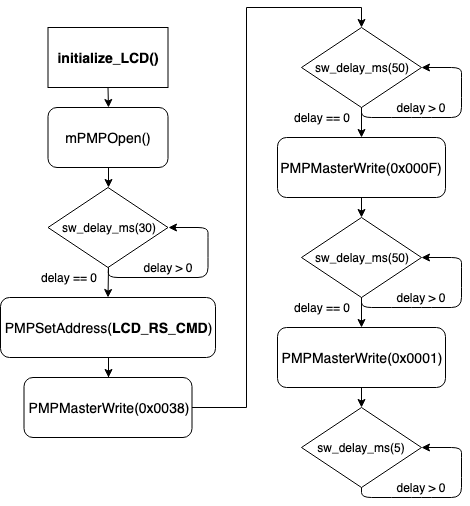
\includegraphics[width=.8\textwidth]{initialize_LCD_CFD.png}
\caption{initialize\_LCD() Control Flow Diagram}
\end{figure}

\begin{figure}[htb]
\centering
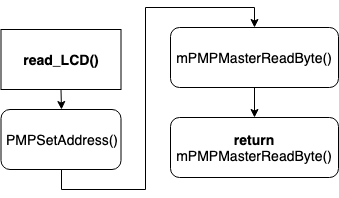
\includegraphics[width=.6\textwidth]{read_LCD_CFD.png}
\caption{read\_LCD() Control Flow Diagram}
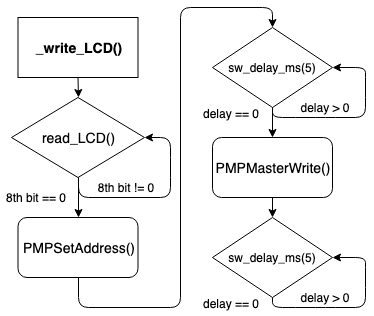
\includegraphics[width=.6\textwidth]{_write_LCD_CFD.png}
\caption{\_write\_LCD() Control Flow Diagram}
\end{figure}

\begin{figure}[htb]
\centering
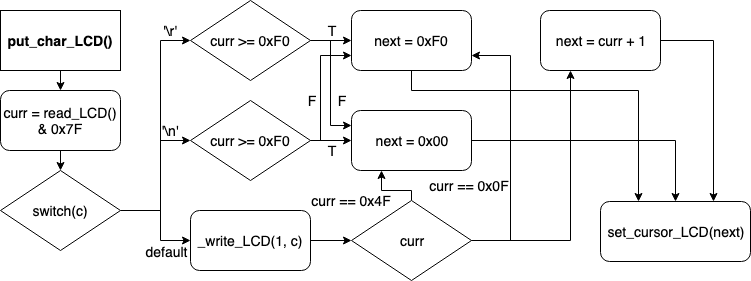
\includegraphics[width=.8\textwidth]{write_char_LCD_CFD.png}
\caption{write\_char\_LCD() Control Flow Diagram}
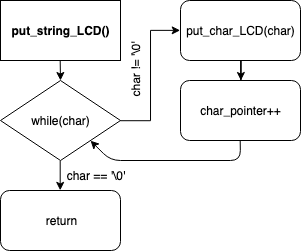
\includegraphics[width=.4\textwidth]{put_string_LCD_CFD.png}
\caption{put\_string\_LCD() Control Flow Diagram}
\end{figure}

\begin{figure}[htb]
\centering
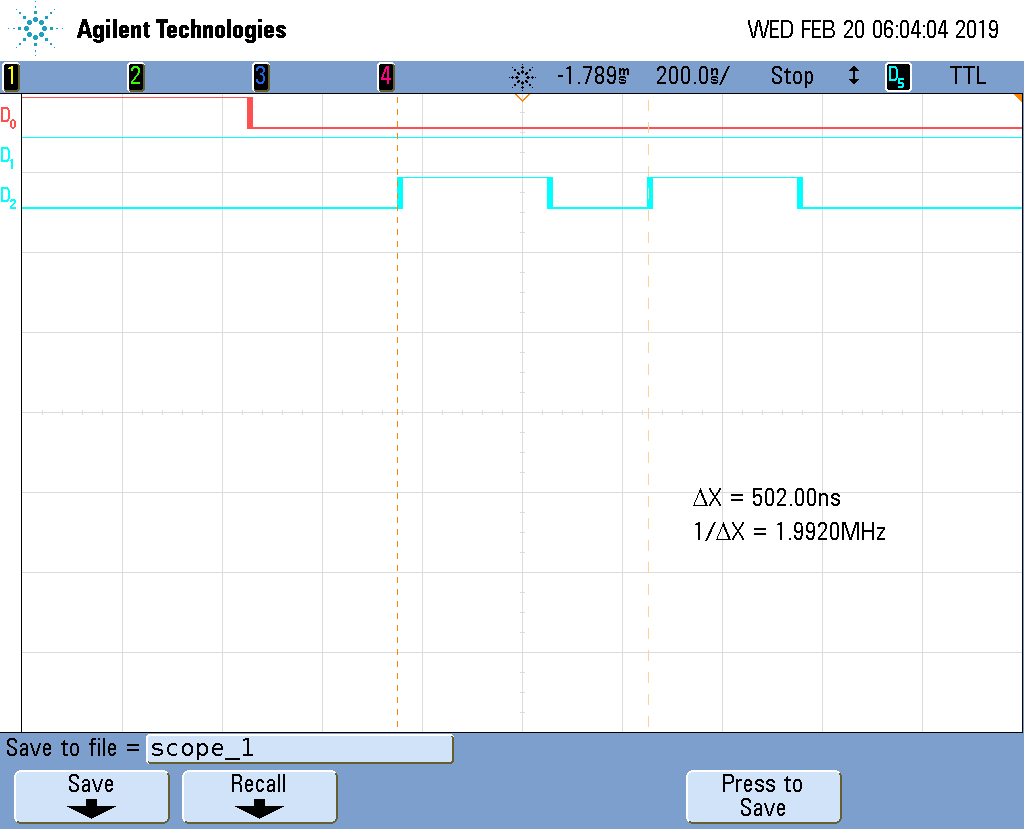
\includegraphics[width=.8\textwidth]{0.png}
\caption{Enable Cycle Time Validation}
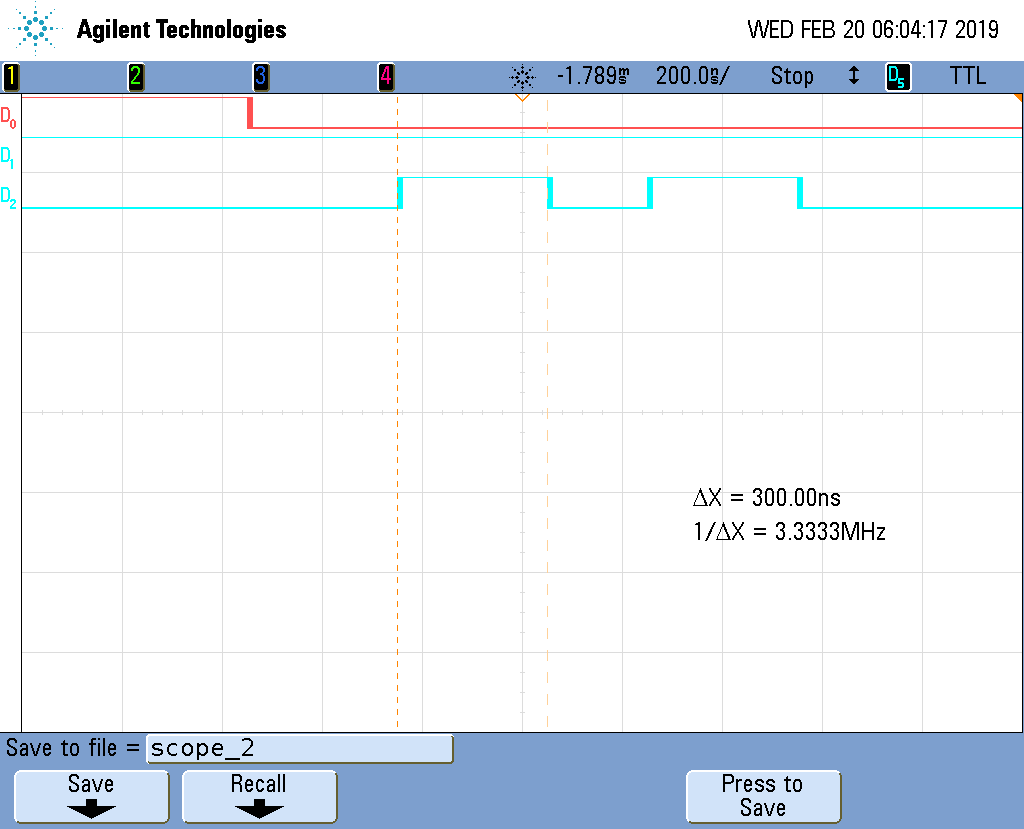
\includegraphics[width=.8\textwidth]{1.png}
\caption{Enable High Pulse Width Validation}
\end{figure}

\begin{figure}[htb]
\centering
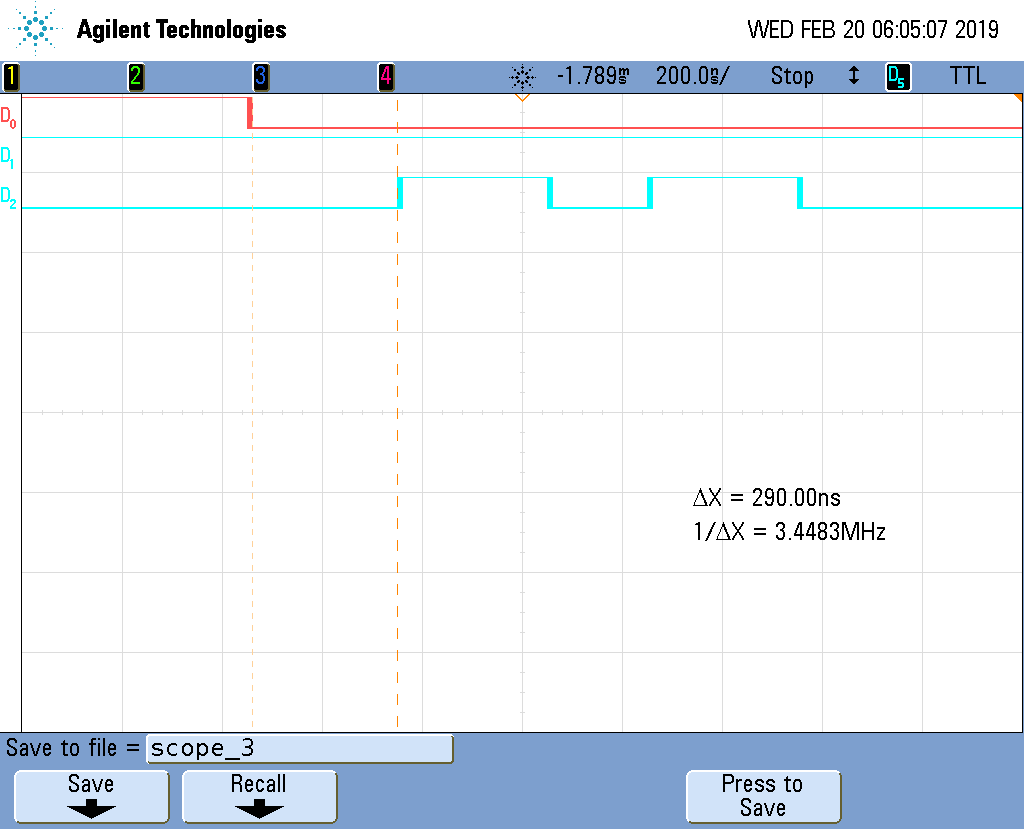
\includegraphics[width=.8\textwidth]{2.png}
\caption{RS, R/W Setup Time Validation}
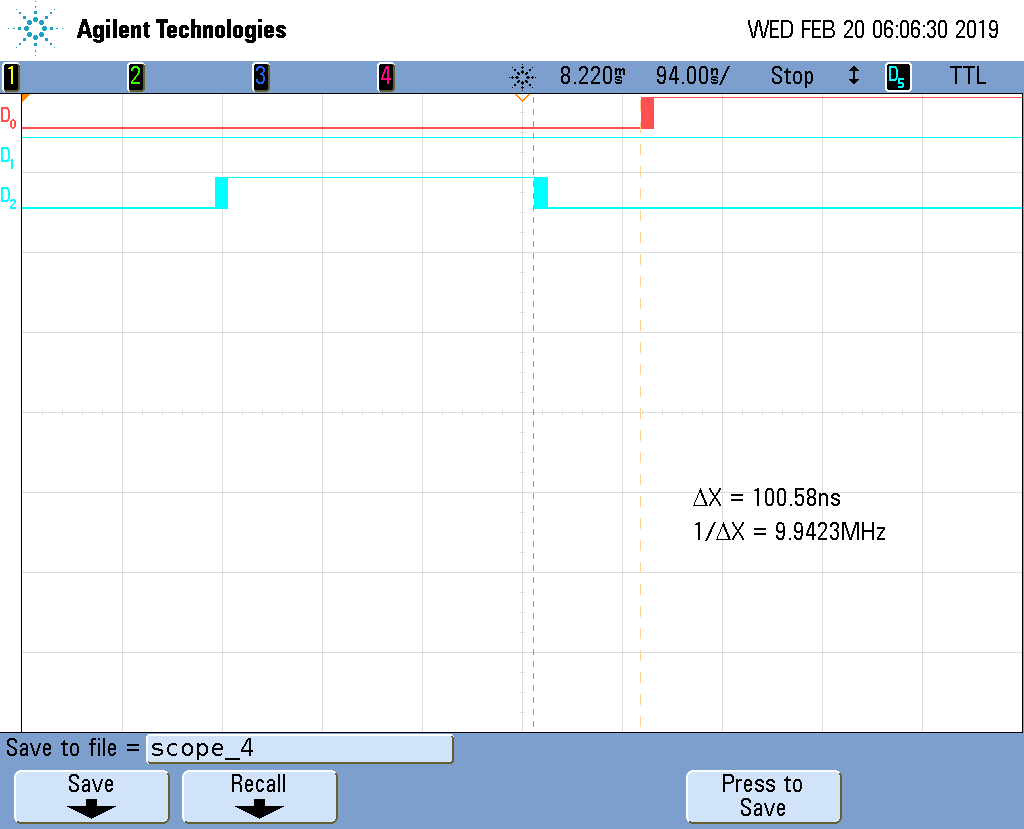
\includegraphics[width=.8\textwidth]{3.png}
\caption{RS, R/W Hold Time Validation}
\end{figure}

\end{document}